\documentclass[11pt,a4paper,oneside]{report}

\usepackage[dvipsnames]{xcolor}
\usepackage{amsmath}
\usepackage{multirow}
\usepackage{caption}
\usepackage{tabularx}
\usepackage{tikz}

\usepackage{listings}

\definecolor{mtypecolor}{HTML}{491b68}
\definecolor{mtypeparamcolor}{HTML}{1e5b0e}
\definecolor{mdatasizecolor}{HTML}{aa5908}
\definecolor{mdatacolor}{HTML}{c40f0f}

\newcommand{\code}{\texttt}

\newcommand*{\xdash}[1][5em]{\rule[0.5ex]{#1}{0.55pt}}
\def\emptycell{\multicolumn{1}{c|}{\xdash}}

\usetikzlibrary{arrows,positioning, shapes.symbols,shapes.callouts,patterns,calc, automata}

\lstdefinelanguage{Kotlin}{
  comment=[l]{//},
  commentstyle={\color{gray}\ttfamily},
  emph={delegate, filter, first, firstOrNull, forEach, lazy, map, mapNotNull, println, return@},
  emphstyle={\color{OrangeRed}},
  identifierstyle=\color{black},
  keywords={abstract, actual, as, as?, break, by, class, companion, continue, data, do, dynamic, else, enum, expect, false, final, for, fun, get, if, import, in, interface, internal, is, null, object, override, package, private, public, return, set, super, suspend, this, throw, true, try, typealias, val, var, vararg, when, where, while},
  keywordstyle={\color{NavyBlue}\bfseries},
  morecomment=[s]{/*}{*/},
  morestring=[b]",
  morestring=[s]{"""*}{*"""},
  ndkeywords={@Deprecated, @JvmField, @JvmName, @JvmOverloads, @JvmStatic, @JvmSynthetic, Array, Byte, Double, Float, Int, Integer, Iterable, Long, Runnable, Short, String},
  ndkeywordstyle={\color{BurntOrange}\bfseries},
  sensitive=true,
  stringstyle={\color{ForestGreen}\ttfamily},
}

\lstset{basicstyle=\footnotesize\ttfamily,breaklines=true}
\lstset{framextopmargin=5pt, framexleftmargin=5pt, framexrightmargin=5pt, framexbottommargin=5pt, frame=bottomline}
\lstset{language=Kotlin, frame=single, gobble=4, tabsize=4, showstringspaces=false}


\begin{document}

%----------------------------------------------------------------------------
\chapter{Runtime Implementation}\label{sect:RuntimeImpl}
%----------------------------------------------------------------------------

	\section{Messaging}
		\subsection{Format}
		
		All messages start with a fixed prefix (\code{MESSAGE}) and end with a line break and their different parts are separated by hyphens. Messages consists of two logical parts: the header and the payload. The former specifies the type of the message and provides other information as type parameters which may be needed to process this kind of message, while the latter carries additional information in a form of a blob and its size in bytes.
		
		\begin{figure}[h]
			\[
				\code{MESSAGE-}%
				\overbrace{\text{\code{%
					\color{mtypecolor}\{Message type\}\color{black}-%
					(\color{mtypeparamcolor}\{Type parameter\}\color{black}-)*%	
				}}}^{Header}%
				\overbrace{\text{\code{%
					\color{mdatasizecolor}\{Data size\}\color{black}-%
					\color{mdatacolor}\{Data\}?%
				}}}^{Payload}%\text{\code{\textbackslash n}}%
			\]
			\caption*{\emph{Structure of the messages}}
		\end{figure}
		
		\paragraph{Type parameters and payload}
		
		The difference between the type parameters and the payload data is that type parameters can be understood and processed without 'unsafe' operations such as java deserialization. Their arity and types are determined by the message type and their values may consist of primitives, strings or enumerations. This -- combined with a size limit on them -- allows the runtime handler to always safely parse, process and optionally route the messages without requiring to understand the potentially unsafe data of the payload.
		
		The data payload on the other hand deals with binary data produced by one of the actors, and as such should only be parsed by the actor clients, which are already equipped with the proper protective capabilities.
		The payloads size (in bytes) is also included in the message for safe message handling.
		
		Both the type parameters and the payload are converted to base~64 strings as to make message formatting and parsing easier -- due to no necessary separator escaping.
		
		\begin{table}[h]
			\centering
			\setlength{\tabcolsep}{8pt}
			\renewcommand{\arraystretch}{1.5}
			\begin{tabularx}{\linewidth}{
				|>{\hsize=0.8\hsize}X|% 
				>{\hsize=0.8\hsize}X|%
				>{\hsize=1.4\hsize}X|%
			  }
				\hline
				 \multicolumn{1}{|c|}{\textbf{Message type}} &%
				 \multicolumn{1}{c|}{\textbf{Parameters}} &%
				 \multicolumn{1}{c|}{\textbf{Payload}} \\ \hline
				
				Start notice & \emptycell & \emptycell \\ \hline
				Shutdown notice & \emptycell & \emptycell \\ \hline
				
				\multirow{2}{*}{Log entry} & Target actor & \multicolumn{1}{c|}{\multirow{2}{*}{\xdash}} \\
					& Log message & \\ \hline
				
				Error report & Error message & \emptycell \\ \hline
				
				\multirow{2}{*}{Challenge result} & Points & \multicolumn{1}{c|}{\multirow{2}{*}{\xdash}} \\
					& Max points & \\ \hline
				
				Match result & Three way result & \emptycell \\ \hline
				Actor binary & Type & Binary (nothing on requests) \\ \hline
				
				\multirow{2}{*}{Proxy call} & \multirow{2}{*}{Target bot} & Target method \\
					& & Call parameters \\ \hline
				
				Call result & Called method & Result data \\ \hline
				
				Bot timeout & \emptycell & \emptycell \\ \hline
			\end{tabularx}
			\caption*{\emph{Type parameters and payloads of message types}}
		\end{table}

		\subsection{Conversion and serialization}
		
			\paragraph{Conversion and deconversion}
		
			Conversion is the process during which domain representation of a message in the form of a Message object is converted into an intermediate state as it gets ready to be sent. Its result is MessageDTO, an object which holds the same header the original message did, but has its payload -- if any were present -- transformed into a processable, base~64 encoded string representation. Deconversion is its inverse operation. It is a distinct process from the general serialization of messages, as to ensure independence between the algorithms use in the two processes.
			
			This loose coupling is beneficial, as conversion is an unsafe routine that only actor clients should conduct. Message (de)conversion is required when dealing with remote proxy calls, and this breakup of concerns allows the runtime handler to parse and route a call request or call result message without attempting to decode its payload containing jvm objects as transformed by standard java serialization. As object (de)serialization is dangerous -- due to the construction of arbitrary large serialization 'bombs' --, it is best to pass these messages to the actor clients who are equipped with proper security measures to safely minister it.

			\paragraph{Serialization and Deserialization}
			
			Serialization takes payload-less messages or converted messages and transforms them to the aforementioned general message format. This includes encoding the message header and concatenating it to the prefix and optional (already converted) payload. This encoding of the header -- and its pair decoding in deserialization -- can be done safely and strictly, as the contents of the header is specified by the message type and its parameters are simple values that can be easily converted to strings.
			
			As all parties require (de)serialization to communicate, the components providing these services are shared across all of them.

		\subsection{Communication}
		
		All messaging is done over point-to-point, full-duplex TCP channels between the actor clients and the runtime handler. These connections are initialized by the clients, who as a command argument receive the host -- usually localhost -- and the port they should connect to. These ports are free ports chosen randomly by the handler and reserved before the start of the clients.
		
		Once these channels have been established, communication should begin as described by the communication model -- starting with the clients requesting the game specific actor binaries.
		
		If a game if finished -- in a normal way or because of errors -- or a communication channel should fail (e.g. due to unexpected crash of an actor), the runtime notifies all (still reachable) clients with shutdown notices. After sending and receiving these, all participants are to assume the game has ended, the clients stop themselves and the handler reports the result of the challenge or match.

		Just like serialization, low level communication is helped by components shared across all members of the runtime model.

	\section{Runtime handler}

	A runtime handler is made up of a couple of active components and passive data structures. Active components are primarily based on their own thread and communicate with each other either through direct calls or the passive structures.
	The are two kinds of these active components, a -- per runtime handler -- singleton control handler, and actor handlers for each actor client runtimes. Passive components come in the form of a control queue and log stores for each actors.
		
		\begin{figure}[h]
			\centering
			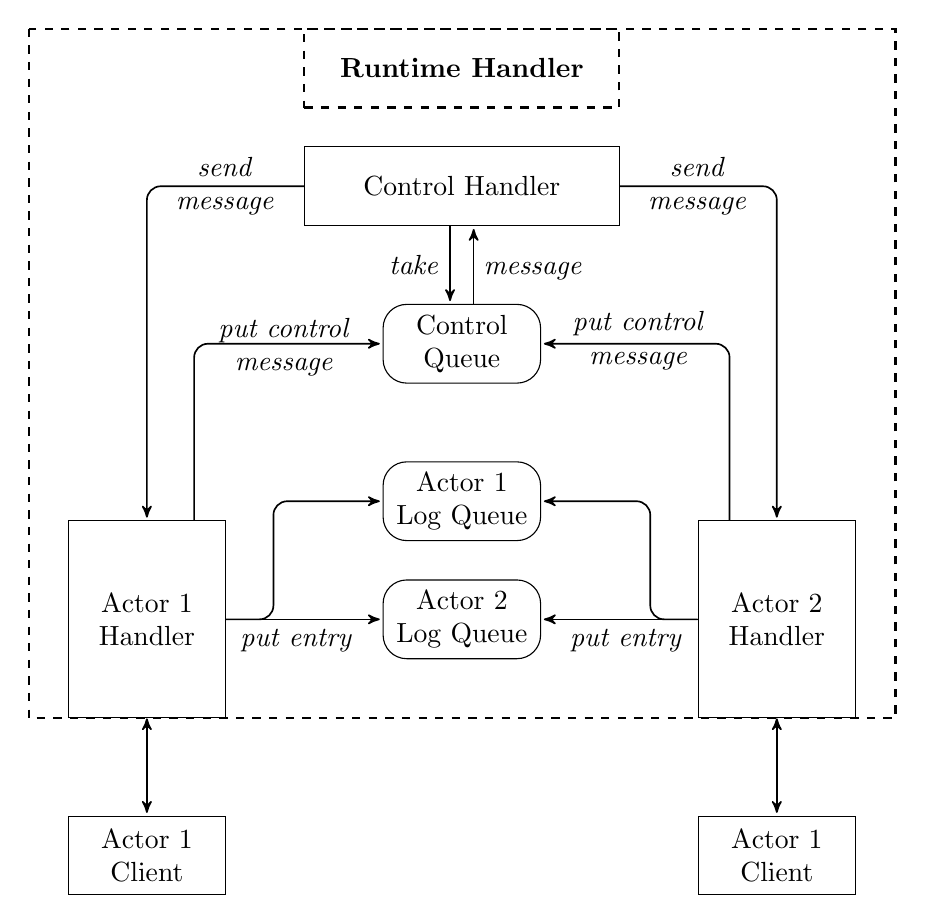
\begin{tikzpicture}[->, >=stealth, rectangle, every node/.style={minimum height=1cm, minimum width=4cm}, node distance=2cm, auto, post/.style={->,shorten >=1pt,>=stealth',semithick}]
			
				\node [draw] (CH) {Control Handler};
				\node [draw] (CQ) [below of = CH, node distance=2cm, minimum width=2cm, align=center, rounded corners=.3cm]
					{Control\\Queue};
				
				\node [draw] (A1LQ)
					[below of = CQ, node distance=2cm, align=center, minimum width=2cm, rounded corners=.3cm]
					{Actor 1 \\ Log Queue};
				
				\node [draw] (A2LQ)
					[below of = A1LQ, node distance=1.5cm, align=center, minimum width=2cm, rounded corners=.3cm]
					{Actor 2 \\ Log Queue};
				
				\node [draw] (A1H)
					[left of=A2LQ, node distance=4cm, align=center, minimum width=2cm, minimum height=2.5cm]
					{Actor 1 \\ Handler};
				
				\node [draw] (A2H)
					[right of=A2LQ, node distance=4cm, align=center, minimum width=2cm, minimum height=2.5cm]
					{Actor 2 \\ Handler};
				
				\node [draw] (A1C)
					[below of=A1H, node distance=3cm, align=center, minimum width=2cm]
					{Actor 1 \\ Client};
				
				\node [draw] (A2C)
					[below of=A2H, node distance=3cm, align=center, minimum width=2cm]
					{Actor 1 \\ Client};
				
				\draw[post] (CH) edge [transform canvas={xshift=-0.15cm}]
					node [left, minimum width=0cm] {\emph{take}} (CQ);
				\draw[post] (CQ) edge [transform canvas={xshift=0.15cm}]
					node [right, transform canvas={yshift=-0.08cm}] [minimum width=0cm] {\emph{message}} (CH);
				
				\draw[post,rounded corners=5pt] (CH) node [align=center, transform canvas={xshift=-3cm}] 
					{\emph{send}\\ \emph{message}} -| (A1H);
				\draw[post,rounded corners=5pt] (CH) node [align=center, transform canvas={xshift=3cm}] 
					{\emph{send}\\ \emph{message}} -| (A2H);
				
				\draw[post,rounded corners=5pt] (A1H.north) ++(.6,0) |-
					node [transform canvas={xshift=1.15cm, yshift=-0.55cm}, align=center]
					{\emph{put control}\\ \emph{message}} (CQ);
				\draw[post,rounded corners=5pt] (A2H.north) ++(-.6,0) |- 
					node [transform canvas={xshift=-1.15cm, yshift=0.55cm}, align=center]
					{\emph{put control}\\ \emph{message}} (CQ);
				
				\draw[post,rounded corners=5pt] (A1H.east) -- ++(.6,0) |- (A1LQ);
				\draw[post] (A1H.east) node [minimum height=0cm, below, transform canvas={xshift=0.9cm}]
					{\emph{put entry}} |- (A2LQ);
				
				\draw[post,rounded corners=5pt] (A2H.west) -- ++(-.6,0) |- (A1LQ);
				\draw[post] (A2H.west) node [minimum height=0cm, below, transform canvas={xshift=-0.9cm}]
					{\emph{put entry}} |- (A2LQ);
				
				\draw[post, <->] (A1H) edge (A1C);
				\draw[post, <->] (A2H) edge (A2C);
				
			    \draw[thick, dashed] (-5.5cm,2cm) rectangle ($(A2H.south east) + (0.5,0)$);
				\node[draw, dashed, thick] (T) [above of=CH, node distance=1.5cm] {\textbf{Runtime Handler}};
				
			\end{tikzpicture}
			\caption*{\emph{Runtime handler simplified component model}\\ \emph{Challenge -- two actors}}
		\end{figure}
		
		\subsection{Control handler}
		
		The control handler is the heart of the runtime handler, as its name implies, it directs the flow of the game and manages the actor handlers. At its core it is a finite--state machine that processes control messages and optionally instructs the actor handlers to send messages based on the actions.
		
		It is important to note that the control messages it consumes are slightly different from the general messages sent between the members of the runtime model, as they have been preprocessed by the actor handlers. The two main changes are that log messages have been removed (they are processed by the actor handlers), and each message contains its source actor. The control handler acquires these messages from the message queue, which acts as a thread--safe buffer between the components. The possible control state are:
		
		\begin{itemize}
			\item \textbf{Connection await} The initial state, it signals that not all actor clients are ready to start as not all have connected or received all the binaries they need.
			
			\item \textbf{Wait for Engine} The engine is working.

			\item \textbf{Wait for Bot} The engine had requested a proxy call, whose result has not been returned from the target bot's actor yet.
			
			\item \textbf{Finished} The game had finished normally. \emph{End}
			
			\item \textbf{Crash} The game finished abnormally due to some error. \emph{End}
		\end{itemize}

		\begin{figure}[h]
			\centering
			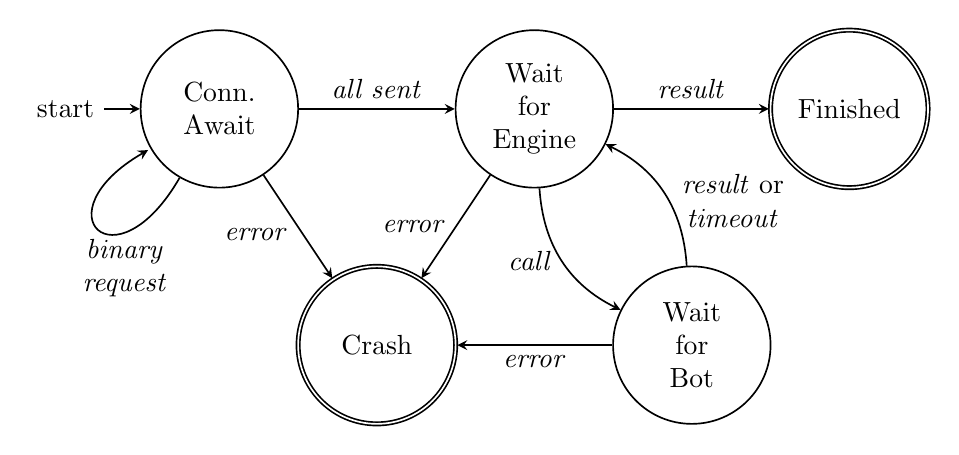
\begin{tikzpicture}[->, >=stealth, node distance=4cm, auto, semithick, state/.style={circle, draw, minimum size=2cm}]
				\pgfmathtruncatemacro{\last}{4}		
		
				\node[state, initial, align=center] (ConnAwait)
					{Conn. \\ Await};
				\draw (ConnAwait) edge [in=210,out=240,loop] node [align=center, xshift=1cm]
					{\emph{binary} \\ \emph{request}} (ConnAwait);
		
				\node[state, right of=ConnAwait, align=center] (WaitEngine) {Wait \\ for \\ Engine};
		
				\node[state, right of=WaitEngine, align=center, accepting] (Done)
					{Finished};
		
				\node[state, below of=ConnAwait, node distance=3cm, align=center, accepting] (Crash)
					at ($(ConnAwait)!0.5!(WaitEngine)$) {Crash};
		
				\node[state, below of=WaitEngine, node distance=3cm, align=center] (WaitBot)
					at ($(WaitEngine)!0.5!(Done)$) {Wait \\ for \\ Bot};
		
				\draw (ConnAwait) edge node {\emph{all sent}} (WaitEngine);
				\draw (WaitEngine) edge node {\emph{result}} (Done);
		
				\draw (ConnAwait) edge node [left, yshift=-0.1cm] {\emph{error}} (Crash);
				\draw (WaitEngine) edge node [left] {\emph{error}} (Crash);
				\draw (WaitBot) edge node [below] {\emph{error}} (Crash);
		
				\draw (WaitEngine) edge [bend right] node [left] {\emph{call}} (WaitBot);
				\draw (WaitBot) edge [bend right] node [right, align=center, xshift=0.1cm, yshift=-0.1cm]
					{\emph{result} or \\ \emph{timeout}} (WaitEngine);
		
			\end{tikzpicture}
			\caption*{\emph{Control state machine}}
		\end{figure}

		To simplify game flow management, the control handler is an extended state machine which allows states to store variables as internal state. This data allows for selective transitions to happen and help store results in the final (accepting) states. Each state may have its own set of parameters as follows: 

		\begin{table}[h]
			\centering
			\setlength{\tabcolsep}{8pt}
			\renewcommand{\arraystretch}{1.5}
			\begin{tabularx}{0.8\linewidth}{
				|>{\hsize=0.7\hsize}X|% 
				>{\hsize1.3\hsize}X|%
			  }
				\hline
				 \multicolumn{1}{|c|}{\textbf{Control state}} &%
				 \multicolumn{1}{c|}{\textbf{Parameters}} \\ \hline
				
				Connection await & sent binaries by receiver client \\ \hline
				Wait for Engine & \emptycell \\ \hline
				Wait for Bot & target bot, called method \\ \hline
				Finished & challenge/match result \\ \hline
				Crash & optional result, error description \\ \hline
			\end{tabularx}
			\caption*{\emph{Parameters of control states}}
		\end{table}

			\paragraph{Game flow}
			
			The controller starts off in the \code{Connection await} state and remains there until all actors have received their required binaries. It keeps track of the sent libraries and after the last of these has been issued, a 'Start notice' message is sent to the engine client, the state is changed to \code{Wait for Engine} and the game starts.
			
			During the game as the engine makes call for which the bots respond, the state is bouncing between \code{Wait for Engine} and \code{Wait for Bot}. As a security measure, the target bot and called method are also stored, so that it can be verified that the right bot answered a call. As per the game model, 'Bot timeout' messages are also possible in the place of 'Call results'.
			
			After the game had come to a conclusion and the engine had sent the proper result message, the state reaches \code{Finished}, where it keeps the game result and stays.
			
			Of course, while in any active state, an error might also happen, in which case the controller changes to \code{Crash} state. Although in this case a game result have not been reported by the engine, the controller might set a valid result anyway, based on the context in which the error occurred. If for example the game crashed due to a runtime exception while executing a code of a bot, the result of the challenge or match will be set to error from that bot -- a result that is processed similarly to the opponent winning in the case of a match, or a 0 point run in the case of a challenge.

		\subsection{Actor handler}

		In contrast to the control handler, separate actor handlers are create for each actors. These composite components are responsible for communicating with the runtime clients, processing incoming messages, storing log entries, and forwarding control messages to the control handler in a digestible format.
		
		Low level communication with the clients is done using a channel, an object which provides a safe, message--aware wrapper for the underlining network sockets. On top of this sits a message handler, which now provides operations based on the type of the clients (engine or bot). This handler is accessed by two components, the already mentioned control handler and the message router receiver. Both of these objects run on their own threads while using the message handler, but due to them only using the sending or receiving capabilities respectively, (and the fact that the underlying architecture is full--duplex capable) these actions can happen independently. The message router receiver's thread can be considered the actor handler's main thread, as it performs most of the tasks of the handler. It blockingly waits for incoming messages, then routes them according their purpose. 

		Control messages get transcribed into the format the control handler can understand and put onto the control queue, from where they will be taken by the control handler. Log messages on the other hand are passed to a log router, an object which puts them into their target's log queue. As game engines have the power to simultaneously send info entries to multiple actors, this might mean more than one overall targets.
		
		Actor handlers are designed to be as reusable as possible when dealing with different types of actors. This means that only the message handler and the log router differ based on actor kind -- as they either must show different sending methods to the outside, or must work fundamentally differently while routing messages --. Also their characteristics are hidden from the other components (except for the control handler) via abstraction achieved by inheritance of a base. 

		\begin{figure}[h]
			\centering
			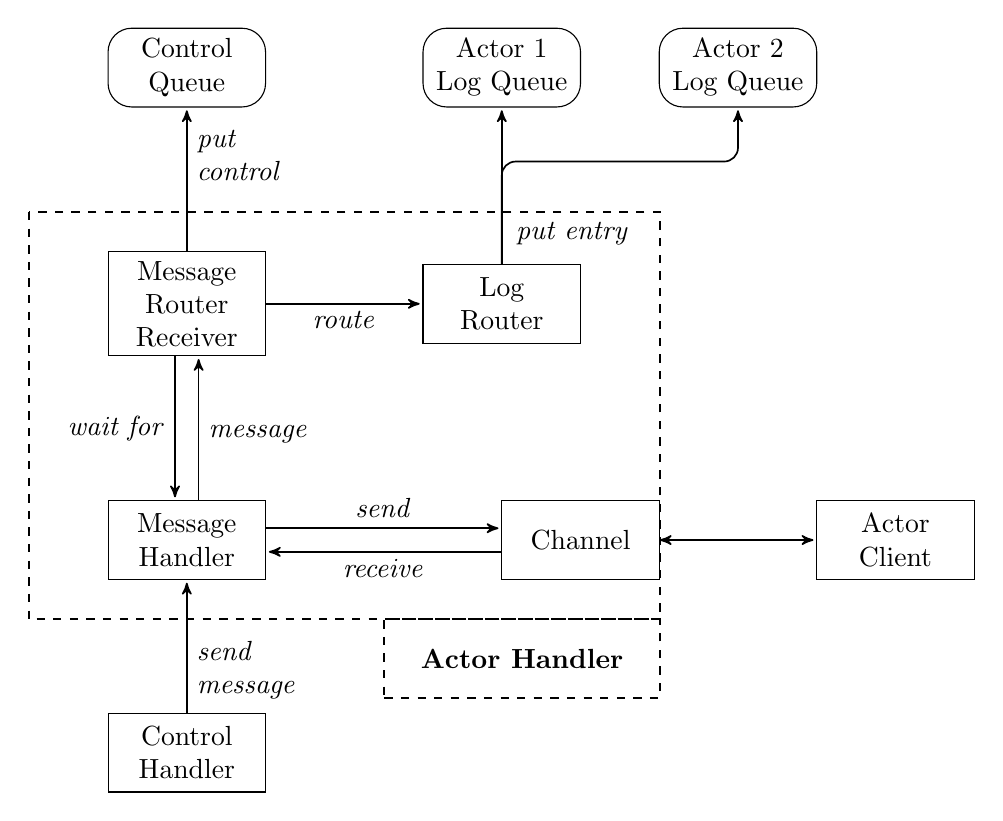
\begin{tikzpicture}[->, >=stealth, rectangle, every node/.style={minimum height=1cm, minimum width=4cm}, node distance=2cm, auto, post/.style={->,shorten >=1pt,>=stealth',semithick}]
			
				\node [draw] (CQ) [minimum width=2cm, align=center, rounded corners=.3cm]
					{Control\\Queue};
				
				\node [draw] (A1LQ)
					[node distance=4cm, right of=CQ, minimum width=2cm, align=center, rounded corners=.3cm]
					{Actor 1\\Log Queue};
				
				\node [draw] (A2LQ)
					[node distance=3cm, right of=A1LQ, minimum width=2cm, align=center, rounded corners=.3cm]
					{Actor 2\\Log Queue};
				
				\node [draw] (MRR)
					[node distance=3cm, below of=CQ, minimum width=2cm, align=center]
					{Message\\Router\\Receiver};
				
				\node [draw] (LR)
					[node distance=4cm, right of=MRR, minimum width=2cm, align=center]
					{Log\\Router};

				\node [draw] (MH)
					[node distance=3cm, below of=MRR, minimum width=2cm, align=center]
					{Message\\Handler};
				
				\node [draw] (C)
					[node distance=5cm, right of=MH, minimum width=2cm, align=center]
					{Channel};
				
				\node [draw] (AC)
					[node distance=4cm, right of=C, minimum width=2cm, align=center]
					{Actor\\Client};
				
				\node [draw] (CH)
					[node distance=2.7cm, below of=MH, minimum width=2cm, align=center]
					{Control\\Handler};
				
				\draw[post] (MRR) edge [right] node [minimum width=0cm, align=left, yshift=0.3cm]
					{\emph{put}\\ \emph{control}} (CQ);
				
				\draw[post] (MRR) edge [below] node [minimum width=0cm, align=center, yshift=0.3cm]
					{\emph{route}} (LR);
				
				\draw[post] (LR) edge [below] node
					[minimum width=0cm, align=center, yshift=-0.1cm, xshift=0.9cm]
					{\emph{put entry}} (A1LQ);
					
				\draw[post,rounded corners=5pt] (LR.north) -- ++(0,1.3) -| (A2LQ.south);
				
				\draw[post] (MRR) edge [transform canvas={xshift=-0.15cm}]
					node [left, minimum width=0cm] {\emph{wait for}} (MH);
				\draw[post] (MH) edge [transform canvas={xshift=0.15cm}]
					node [right, transform canvas={yshift=-0.08cm}, minimum width=0cm] {\emph{message}} (MRR);
				
				\draw[post] (MH) edge [transform canvas={yshift=0.15cm}]
					node [above, minimum width=0cm, yshift=-0.25cm] {\emph{send}} (C);
				\draw[post] (C) edge [transform canvas={yshift=-0.15cm}]
					node [below, transform canvas={yshift=0.3cm}, minimum width=0cm] {\emph{receive}} (MH);
				
				\draw[post] (CH) edge [right] node [minimum width=0cm, yshift=-0.3cm, align=left]
					{\emph{send}\\ \emph{message}} (MH);
				
				\draw[post, <->] (C) edge (AC);
				
				\draw[thick, dashed] ($(MRR.north west) + (-1,0.5)$) rectangle ($(C.south east) + (0,-0.5)$);
				\node[draw, dashed, thick] (T) [below = of C.east, anchor=east, minimum width=3.5cm, yshift=0.495cm, xshift=0.015cm]
					{\textbf{Actor Handler}};
				
			\end{tikzpicture}
			\caption*{\emph{Actor handler model} \\ \emph{Challenge -- two actors}}
		\end{figure}		
		
	\section{Actor runtime}

	The structure of actor runtimes is fairly simple and is largely identical between engine-- and bot clients. Their core component is the 'client', which provides the logic necessary to manage the actor assigned to them, and therefore of course contains actor role (engine or bot) specific code. The rest of the components involved in the communication process are equivalent in each cases. The client is based on three active objects all running on separate threads, a message receiver, a message sender and the aforementioned client. These elements are communicating with each other -- in a one--way manner -- over blocking queues.
		
	\begin{figure}[h]
		\centering
		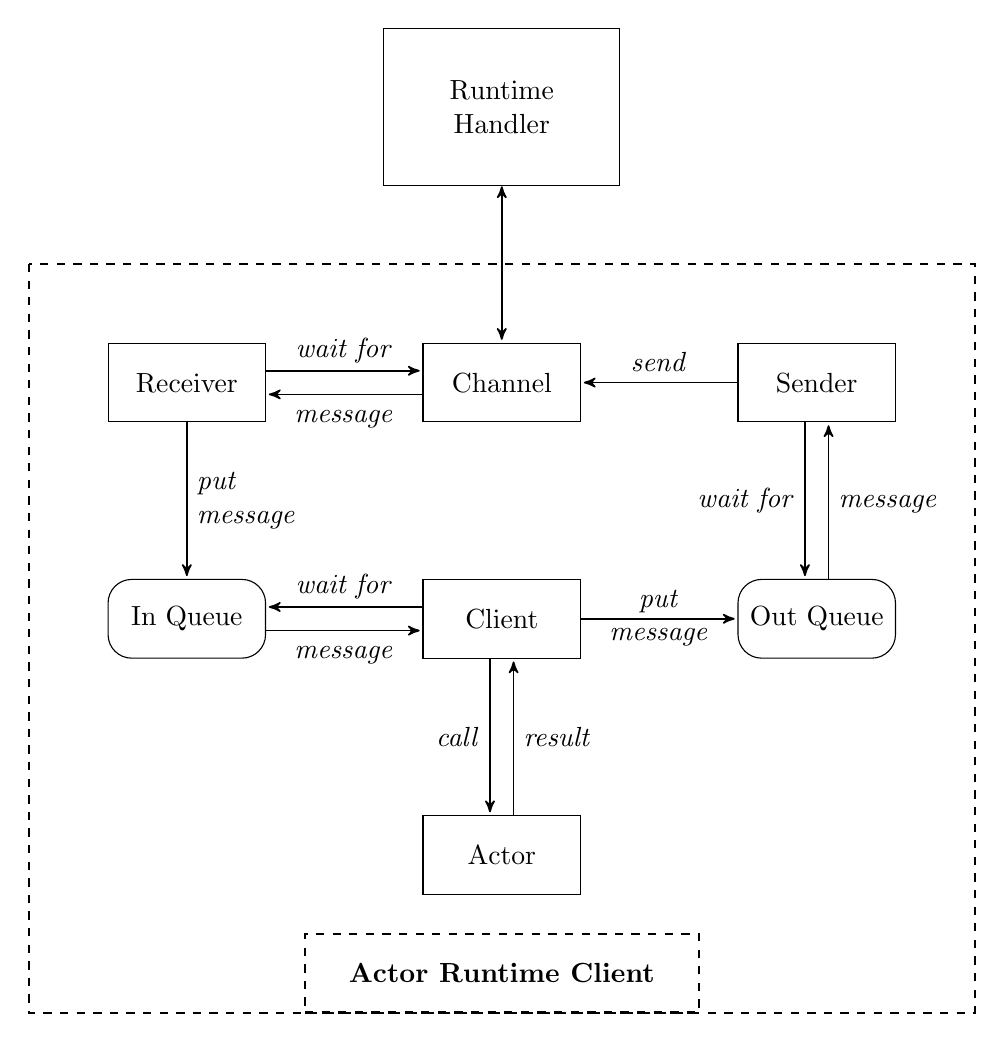
\begin{tikzpicture}[->, >=stealth, rectangle,
							every node/.style={minimum height=1cm, minimum width=2cm, align=center},
							node distance=3cm, auto,
							post/.style={->,shorten >=1pt,>=stealth',semithick},
							passive/.style={rounded corners=.3cm}]
		
			\node [draw] (RH) [minimum width=3cm, minimum height=2cm] {Runtime\\Handler};
			
			\node [draw] (C) [below of=RH, node distance=3.5cm] {Channel};
			
			\node [draw] (R) [left of=C, node distance=4cm] {Receiver};
			
			\node [draw] (S) [right of=C, node distance=4cm] {Sender};
				
			\node [draw, passive] (In) [below of=R] {In Queue};
				
			\node [draw, passive] (Out) [below of=S] {Out Queue};
				
			\node [draw] (CL) [below of=C] {Client};
				
			\node [draw] (A) [below of=CL] {Actor};
				
			\draw[post] (RH) edge [<->] (C);
			 
			\draw[post] (R) edge [transform canvas={yshift=0.15cm}]
				node [above, yshift=-0.25cm] {\emph{wait for}} (C);
			\draw[post] (C) edge [transform canvas={yshift=-0.15cm}]
				node [below, yshift=0.2cm] {\emph{message}} (R);
			
			\draw[post] (S) edge node [above, yshift=-0.25cm] {\emph{send}} (C);
			
			\draw[post] (R) edge node [align=left, minimum width=0cm] {\emph{put} \\ \emph{message}} (In);
			
			\draw[post] (S) edge [transform canvas={xshift=0-.15cm}]
				node [left, align=right, minimum width=0cm] {\emph{wait for}} (Out);
			\draw[post] (Out) edge [transform canvas={xshift=0.15cm}]
				node [right, align=left, minimum width=0cm, yshift=-0.05cm] {\emph{message}} (S);
							
			\draw[post] (CL) edge [transform canvas={yshift=0.15cm}]
				node [above, yshift=-0.25cm] {\emph{wait for}} (In);
			\draw[post] (In) edge [transform canvas={yshift=-0.15cm}]
				node [below, yshift=0.2cm] {\emph{message}} (CL);
				
			\draw[post] (CL) edge node [above, yshift=-0.5cm] {\emph{put}\\ \emph{message}} (Out);
					
			\draw[post] (CL) edge [transform canvas={xshift=0-.15cm}]
				node [align=right, left, minimum width=0cm] {\emph{call}} (A);
			\draw[post] (A) edge [transform canvas={xshift=0.15cm}]
				node [align=left, right, minimum width=0cm] {\emph{result}} (CL);
							
			\draw[thick, dashed] ($(R.north west) + (-1,1)$) rectangle ($(A.south east) + (5,-1.5)$);
			\node[draw, dashed, thick] (T)
				[below of = A, node distance=1.5cm, minimum width=5cm]
				{\textbf{Actor Runtime Client}};
								
		\end{tikzpicture}
		\caption*{\emph{Actor runtime client model}}
	\end{figure}
	
	The receiver waits for messages over the communication channel, processes them and places them in 'In queue', from where the client can get them. It may also initiate the exit of the client if a shutdown notice is received. Likewise, the sender sends messages placed in the 'Out queue' by the client.
	
		\subsection{Base client}

			As the client's workflow is dependent on the actor's type it is managing, it is realized as two different classes -- the \code{EngineClient} and the \code{BotClient} --, but many common functions are outsources from these to shared dependencies.

			\subsubsection*{Class loading and security}
		
			The most important job of all actor clients is the provision of a safe runtime environment where the actor's and the game api's inherently untrusted code may be executed. This is supported by the standard solutions provided by the java virtual machine. The heart of guarding valuable resources -- such as files or \mbox{I/O} capabilities, is the strict separation of safe-- and unsafe code with their respective permissions assigned.
			
			Safe code is constituted by all the sources of the runtime client and its dependencies such as java libraries used -- effectively the whole codebase. This partition is granted all possible permissions using a policy file, which is -- with the enforcing security manager -- put into effect via program arguments passed to the jvm.

			\begin{center}
				\begin{minipage}{11cm}
					\begin{lstlisting}[language=Java, title={\code{client.policy}}]
	   grant codeBase "file:${trusted.codebase}" {
		   permission java.security.AllPermission "", "";
	   };
					\end{lstlisting}
				\end{minipage}
			\end{center}
		
			This policy grants all permissions to classes whose source URI matches the the file path also set as a vm argument through \code{-Dtrusted.codebase}. This property is in turn set by the starter script to the executable jar's path that not only contains the actor client but also all of its necessary properties as well.
			
			As a security manager is installed, other code sources have no granted permissions, therefore all other (unsafe) code parts need only not be marked from the same source.
			
		\subsection{Internal logging}
		
	\section{Engine actor runtime}

		\subsection{Initialization}

	\section{Bot actor runtime}
	
		\subsection{Initialization}

	\section{Remote invocation}

\end{document}






